
\section{Modélisation et calculs géométriques\label{sec:model_geometric}}

La modélisation des systèmes robotiques
se base sur la théorie mécanique classique des solides
rigides indéformables.
Les robots sont vus comme une succession de solides rigides 
liés les uns aux autres par des articulations.

Le problème est ici de définir la relation entre 
l'état de ces articulations et l'état des solides du robot et 
les repères de références qui leurs sont attachés 
dans l'espace tridimensionnel.
L'intégration au cours du temps de l'état géométrique du robot 
permet d'en déduire son déplacement dans le monde cartésien.

Il est à noter que le vocabulaire de \og chaine et 
modèle \textit{cinématique} \fg et \og modèle \textit{cinématique} 
inverse \fg est souvent rencontré en lieu et place 
de \og \textit{géométrique} \fg.
L'étude des vitesses et l'estimation de l'état cinématique du robot 
ne sont pas abordés dans cette partie. 
En conséquence, le terme \og \textit{géométrique} \fg est ici préféré.\\

Contrairement aux robots à roues, la modélisation de la géométrie
des robots à pattes est indispensable à l'estimation de leurs déplacements.
Par définition, leurs mouvements sont créés par l'échange 
continuel des solides du robot en contact avec le sol.
La modélisation du contact et du changement de pied de support 
est ainsi particulièrement importante.

\subsection{Degrés de liberté et définitions}

Une notion centrale pour la suite est le concept de degré de liberté :

\begin{definition}
    Le vecteur des degrés de liberté d'un système mécanique (\textit{Degrees Of Freedom}, DOF)
    noté $\bm{q} = \{q_i \in \mathbb{R}\} \in \mathbb{R}^n$ est un paramétrage de taille minimale
    et indépendant permettant de décrire les configurations géométriques atteignables
    (position et orientation) du système dans l'espace.
\end{definition}

Typiquement, un solide dans l'espace tridimensionnel possède six degrés de liberté.
Trois degrés de liberté définissant la position du repère lié au solide dans le repère 
de référence et trois degrés de liberté d'orientation fixant la rotation entre 
ces deux repères.

En toute généralité, une articulation reliant deux solides définit un
ensemble de contraintes sur le mouvement relatif de ces deux corps, 
en rotation et ou en translation. 
Elle engendre alors plusieurs degrés de liberté au système.
\begin{definition}
    Soit deux solides rigides $prec$ et $suiv$ liés respectivement 
    aux repères $\mathfrak{R}_{prec}$ et $\mathfrak{R}_{suiv}$.
    Sans contrainte, la transformation spatiale passant du repère
    $\mathfrak{R}_{prec}$ au repère $\mathfrak{R}_{suiv}$ possède
    six degrés de liberté.
    On dit que les deux solides sont reliés par une articulation si
    la transformation spatiale passant de $\mathfrak{R}_{prec}$ 
    à $\mathfrak{R}_{suiv}$ possède $n \in [1,5]$ degrés de liberté.
    Elle est alors paramétrée par un ensemble minimal et indépendant $\bm{q} \in \mathbb{R}^n$.
\end{definition}

Dans le cadre de nos robots humanoïdes, toutes les articulations
mécaniques sont en rotation. 
Dans la suite, à l'exception de la base flottante 
(voir \ref{sec:modele_topologie}), toutes les articulations 
n'engendreront qu'un unique degré de liberté en rotation.

\subsection{Topologie mécanique\label{sec:modele_topologie}}

Du point de vue du modèle géométrique, les systèmes mécaniques et robotiques se répartissent 
en deux grandes catégories distinctes : les topologies sans boucle cinématique (en boucle ouverte)
et les topologies possédant au moins une boucle cinématique (en boucle fermée).

Par exemple, un bras manipulateur dont chaque segment mécanique 
est connecté au segment précédant par une articulation ne possède 
pas de boucle cinématique. 
A contrario, les robots parallèles ou les systèmes 
en trapèze sont en boucle cinématique fermée.
Plus formellement :

\begin{definition}
    Un système mécanique est en boucle cinématique fermée si et seulement si
    le nombre de degrés de liberté effectif du système est strictement 
    inférieur à la somme des degrés de liberté générée par chacune de ses articulations.
    Sinon, le système est dit sans boucle ou en boucle ouverte.
\end{definition}
Chaque boucle cinématique ajoute des contraintes géométriques réduisant
le nombre de degrés de liberté réels du système.\\

La topologie des systèmes sans boucle se modélise de manière classique 
par un arbre avec les caractéristiques suivantes :
\begin{itemize}
    \item La racine de l'arbre est confondue et alignée avec l'origine du monde.
    \item Les nœuds sont les repères liés à chaque solide rigide composant le robot.
    \item Les arrêtes sont les articulations représentant un degré de liberté et
    contenant deux transformations géométriques. 
    La première transformation passe du repère lié au solide parent au point d'accroche
    de l'articulation sur le solide parent. 
    La seconde transformation est une rotation d'angle $q_i$ passant du point 
    d'accroche de l'articulation sur le solide parent au repère lié au solide enfant.
\end{itemize}

Cette modélisation est bien adaptée à la représentation d'un robot fixe tel
qu'un bras manipulateur où la base du robot est confondue avec l'origine
du monde. 
Dans le cas d'un robot mobile, il est nécessaire d'y ajouter 
une \textit{base flottante} afin de tenir compte du déplacement du robot
dans le monde. 

Plus précisément, une racine virtuelle ou base flottante est fixée
sur un solide du robot. 
L'arbre mécanique du robot est alors décrit à partir de cette racine virtuelle.
De plus, une articulation à six degrés de liberté représentant 
un déplacement non contraint doit être introduit entre 
la racine à l'origine du monde et la base flottante.
L'intérêt est de pouvoir placer dans le monde la base flottante
à n'importe quelle position et orientation souhaitées.

Néanmoins, il est intéressant du point de vue de l'implémentation
d'assurer qu'une articulation n'engendre toujours qu'un unique degré de liberté
par souci d'homogénéité.

En conséquence, six articulations unitaires (trois translations et trois rotations) 
sont ajoutées entre la racine de l'arbre à l'origine du monde et la base flottante
située sur le robot. 
Enfin, les six articulations sont reliées par des solides virtuels de
taille et de masse nulles.

En pratique, l'ordre de ces articulations est important et
les trois rotations forment ainsi trois angles de Cardan (Tait-Bryan).
L'ordre est le suivant :
\begin{enumerate}
    \item Translation selon $\vec{\bm{x}}$.
    \item Translation selon $\vec{\bm{y}}$.
    \item Translation selon $\vec{\bm{z}}$.
    \item Rotation autour de $\vec{\bm{z}}$.
    \item Rotation autour de $\vec{\bm{y}}$.
    \item Rotation autour de $\vec{\bm{x}}$.
\end{enumerate}
À noter que même si ces angles de Cardan sont sujets aux singularités
bien connues, l'utilisation qui en est faite pour orienter le robot humanoïde
en position debout ne se rapproche jamais de ces singularités.

Enfin, plusieurs emplacements sur le robot sont possibles 
pour le choix de la racine (virtuelle) de l'arbre mécanique :
\begin{itemize}
    \item Au niveau du tronc (\textit{trunk}).
    \item Au niveau du centre du pied gauche (\textit{left\_foot\_tip}).
    \item Au niveau du centre du pied droit (\textit{right\_foot\_tip}).
\end{itemize}

À noter que conformément au schéma \ref{fig:humanoid}, 
un point mécanique important du modèle de nos robots
est que les trois axes de rotation de la hanche gauche 
et droite sont concourants. 
De la même manière, les deux axes de rotation
de la cheville ainsi que les deux axes de rotation des épaules 
s'intersectent également en un point.

\begin{figure}[htb!]
    \begin{center}
        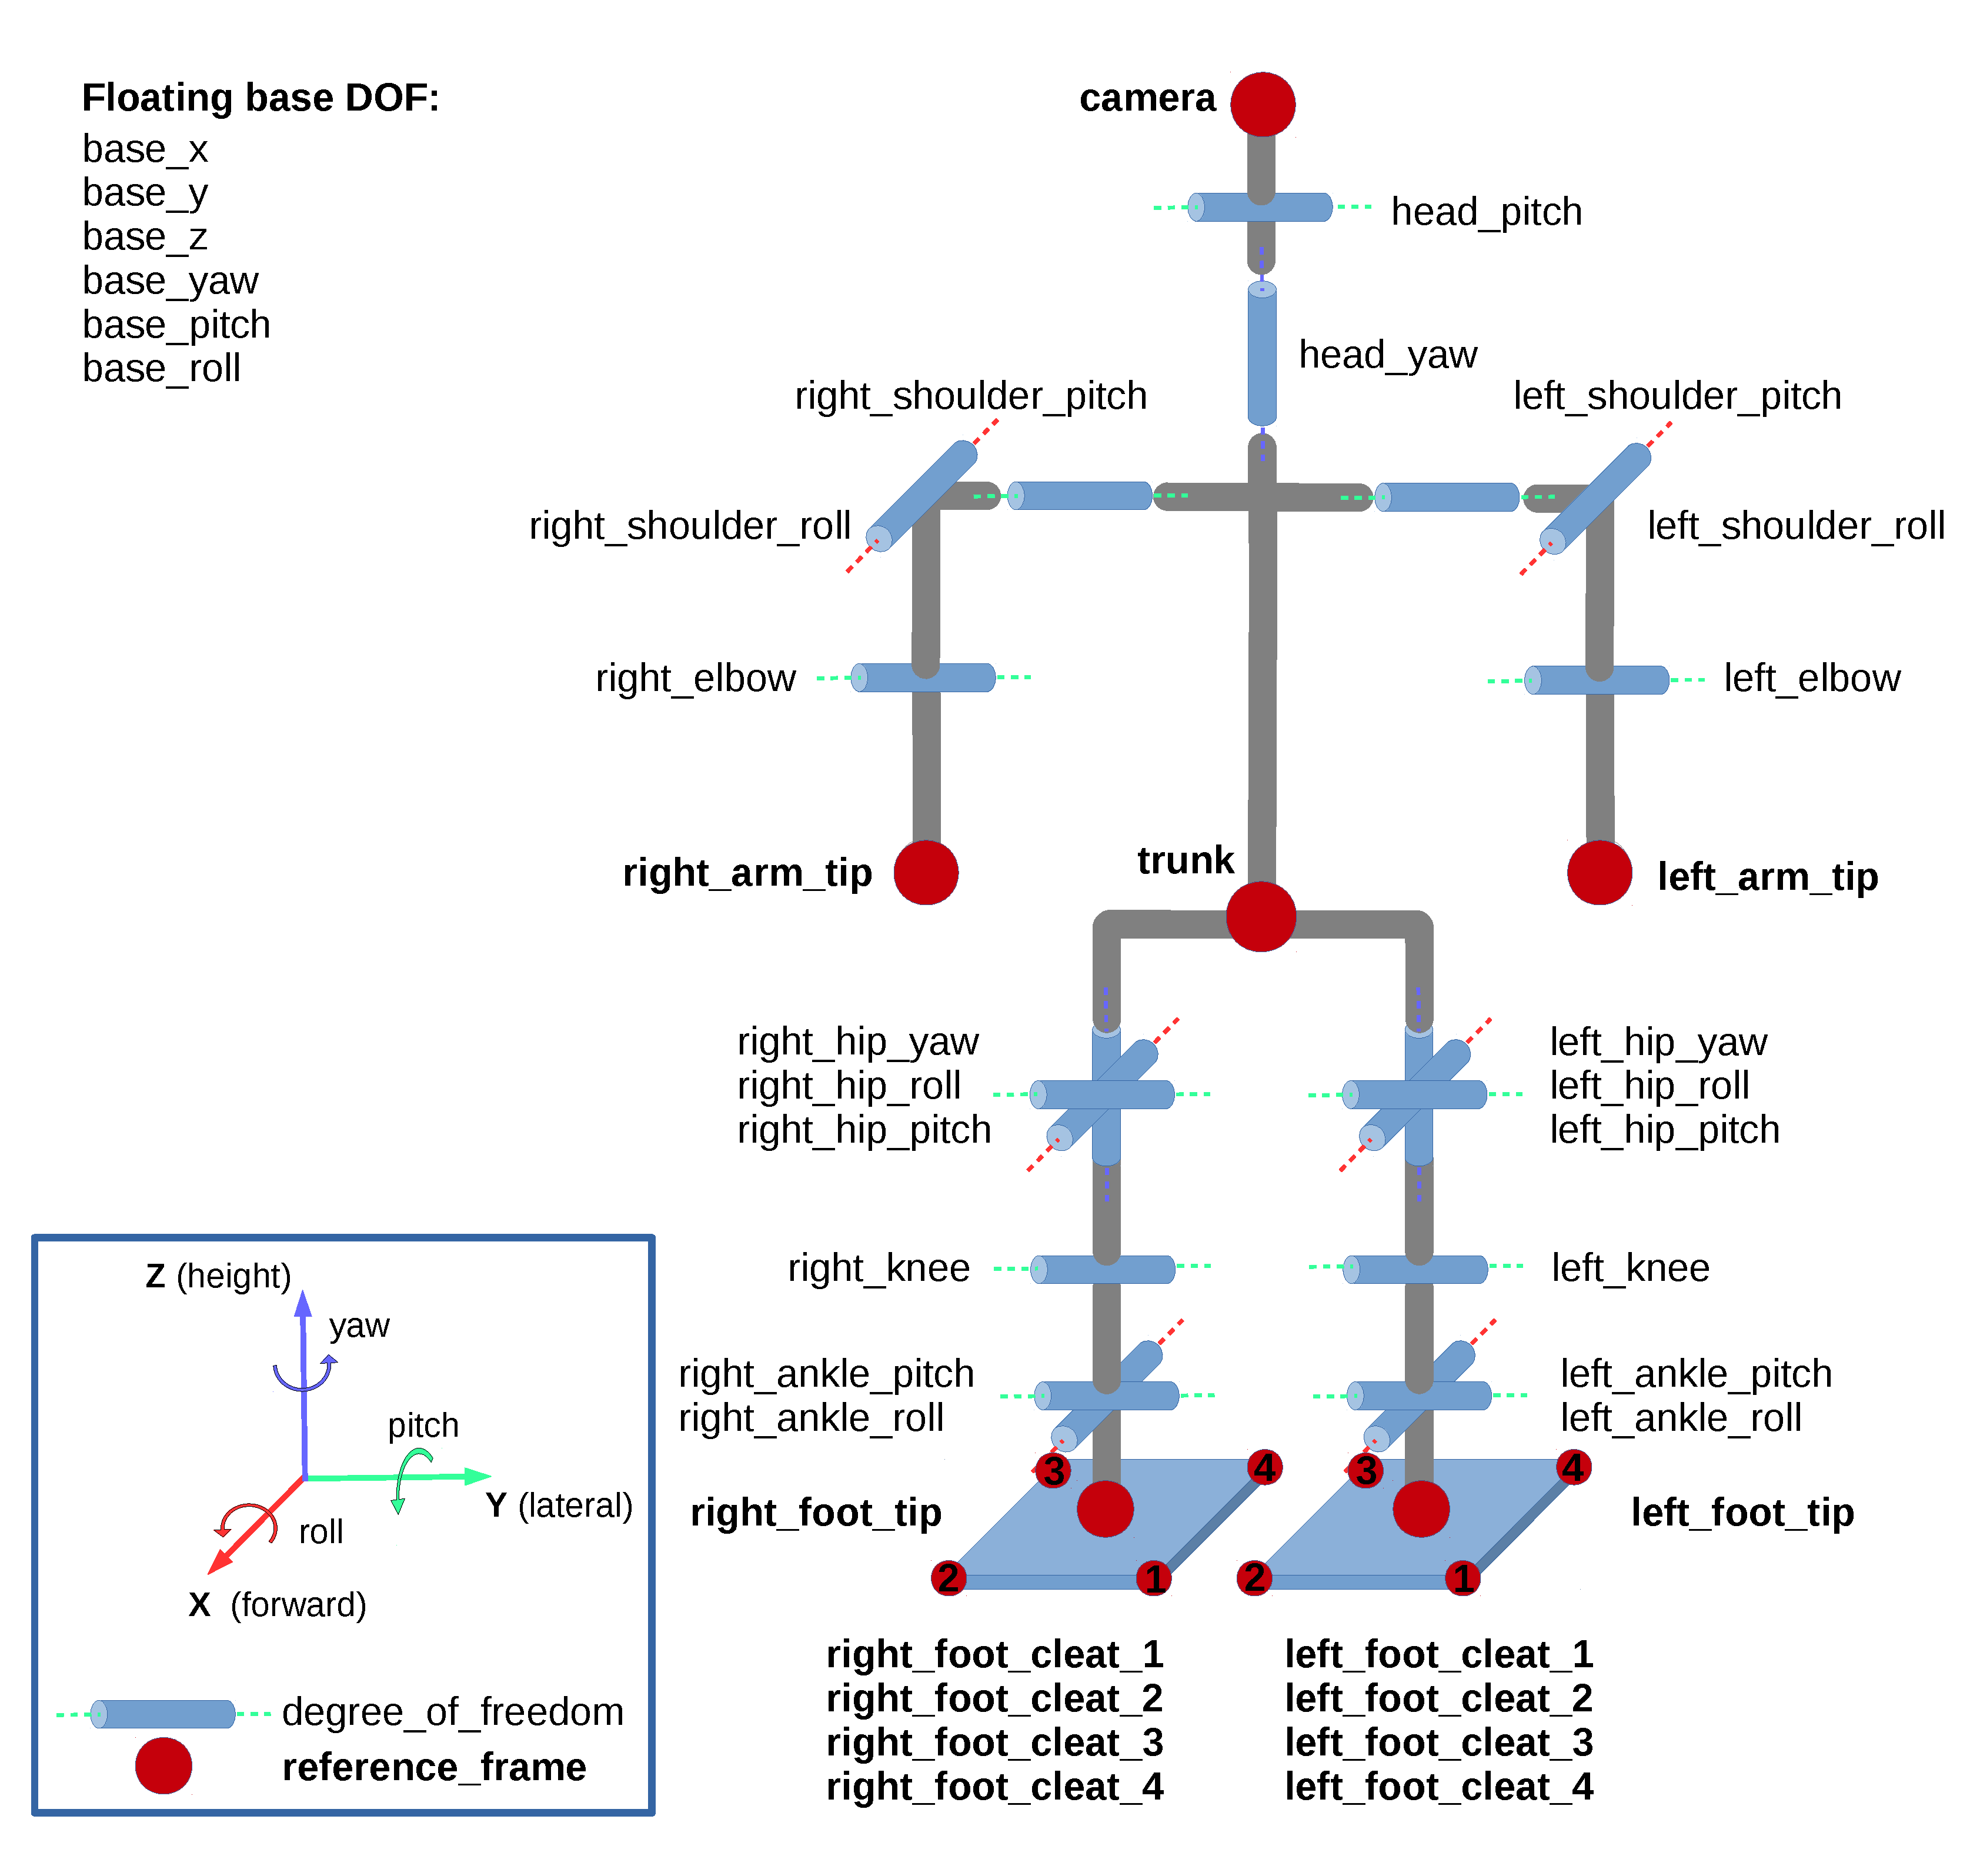
\includegraphics[type=pdf,ext=.pdf,read=.pdf,width=\linewidth]{../schema/humanoid}
        \caption{\label{fig:humanoid}Topologie mécanique et convention 
        de nommage géométrique du robot Sigmaban. 
        Tous les degrés de liberté des articulations et de la base flottante 
        ainsi que les principaux repères de références sont représentés.}
    \end{center}
\end{figure}

\subsection{Pied de support\label{sec:support_foot}}

En toute généralité, la base flottante permet de placer
le modèle du robot humanoïde dans n'importe quelle position et orientation
de l'espace.
Mais en pratique, seules les configurations où le robot est stable debout 
en position de marche ou de tir sont considérées.
En permanence, il est supposé que le robot possède au moins 
un pied au sol et qu'il n'est en contact avec le sol qu'avec ses pieds.

Les pieds du robot son modélisés de la manière suivante :
\begin{itemize}
    \item Les bords et les crampons des pieds ne sont pas considérés.
    \item On dit qu'un pied est posé sur le sol si l'altitude $z$
    (dans le repère du monde) du repère attaché au pied 
    \textit{left\_foot\_tip} ou \textit{right\_foot\_tip} 
    (voir les repères de références dans dans le tableau \ref{tab:frames})
    est nulle.
    \item Le sol est supposé parfaitement non glissant. 
    La position d'un pied en contact avec le sol est donc fixe 
    dans le repère du monde.
    \item Les pieds ne sont pas nécessairement plat sur le sol 
    (voir l'estimation de l'état du robot dans la section \ref{sec:estimation_etat}).
    \footnote{Le robot marche en pratique sur de l'herbe artificielle. 
    Malgré ses crampons, l'herbe rapportée au poids et à la taille du robot tend à incliner légèrement le pied.
    Cette inclinaison est théoriquement mesurable en comparant la mesure de l'IMU 
    et le modèle géométrique direct de la jambe de support.}
\end{itemize}

\begin{definition}
    On dit que le robot humanoïde est en état de simple support (\textit{SS}) quand
    un seul de ses pieds est posé sur le sol. 
    Il est alors soit en simple support gauche (\textit{Left Support Foot}, \textit{LSS}) 
    s'il s'agit de son son pied gauche, soit en simple support droit 
    (\textit{Right Support Foot}, \textit{RSS}) s'il s'agit de son pied droit.
    On dit que le robot est en état de double support (\textit{DS}) quand ses deux pieds
    sont posés sur le sol.
\end{definition}
L'état de support du robot est alors un élément de $\{DD, LSS, RSS\}$.

La modélisation topologique du robot est la suivante :
\begin{itemize}
    \item En état de simple support gauche, respectivement droit,
    la topologie du robot est modélisée en plaçant la racine virtuelle
    au niveau du pied gauche (\textit{left\_foot\_tip}), respectivement droit 
    (\textit{right\_foot\_tip}), fixé par rapport à l'origine du monde.
    \item En état de double support, la racine est placée au niveau du 
    pied de support utilisé lors du dernier état de simple support
    ou du pied gauche par défaut.
    \item Deux modèles géométriques distincts du robot sont ainsi considérés.
    Le modèle de support gauche et le modèle de support droit.
\end{itemize}
Le degré de liberté en translation $z$ de la base flottante
est donc en pratique toujours nul.

\subsection{Repères et conventions\label{sec:model_conventions}}

\begin{figure}[htb]
    \begin{center}
        \begin{minipage}{0.6\linewidth}
            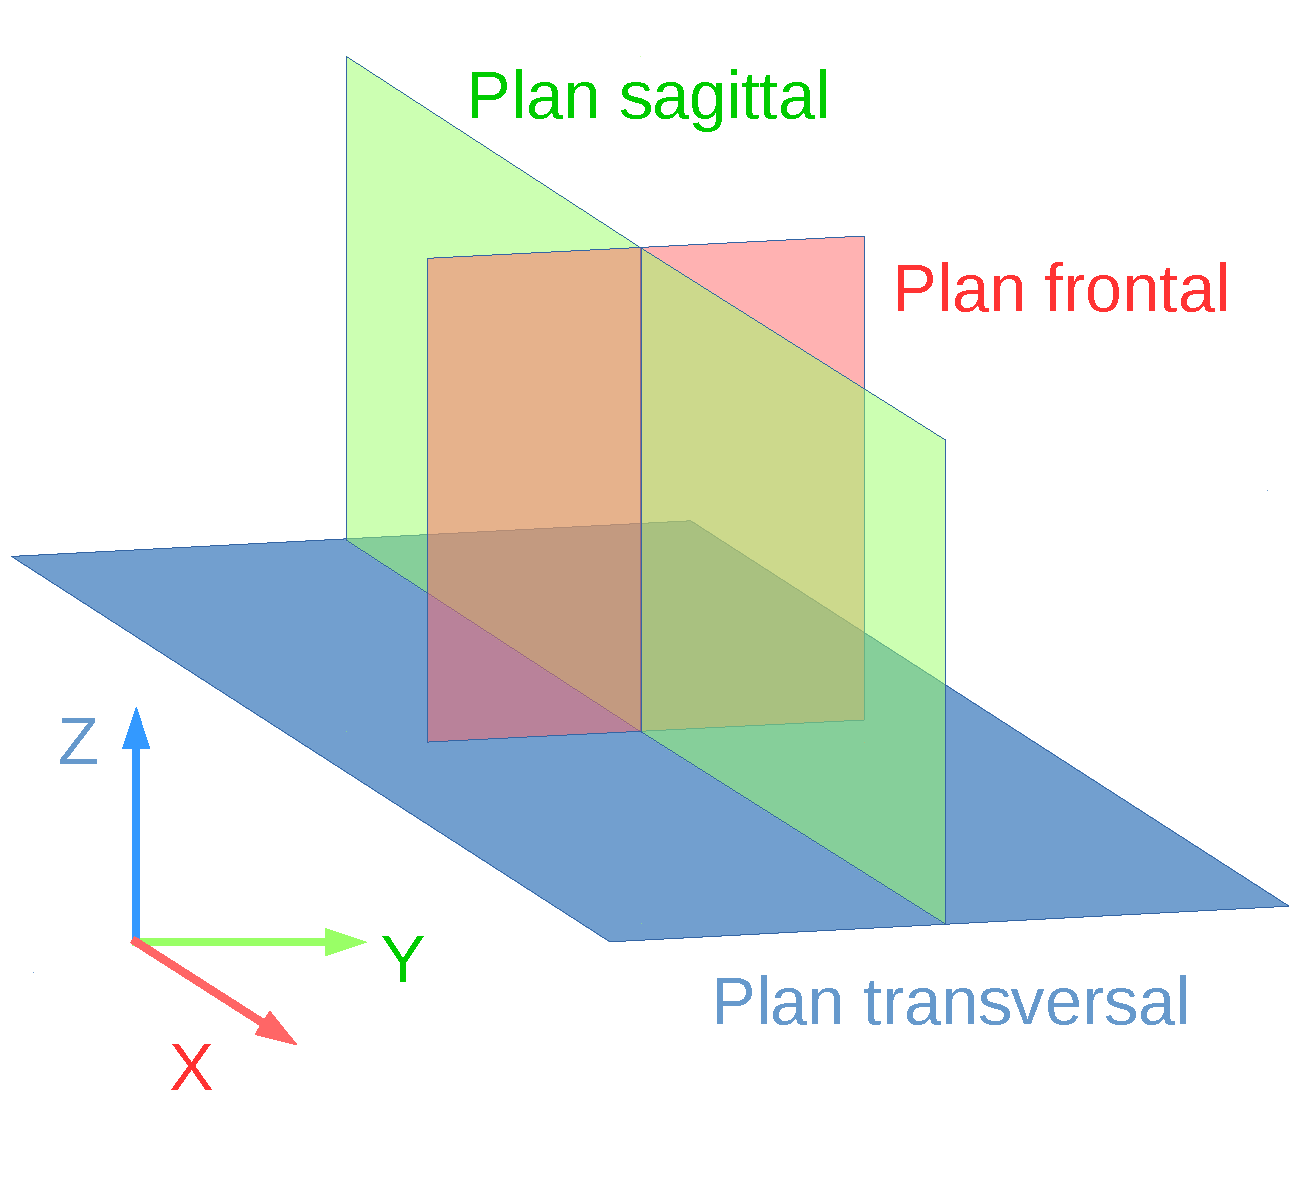
\includegraphics[type=pdf,ext=.pdf,read=.pdf,width=\linewidth]{../schema/planes}
        \end{minipage}
        \begin{minipage}{0.3\linewidth}
            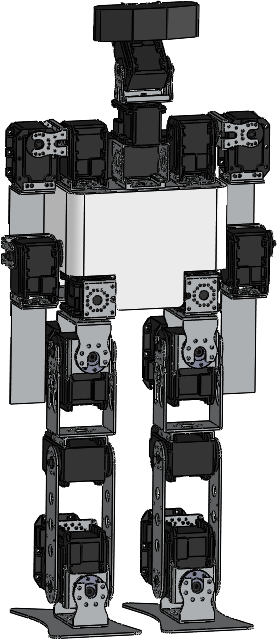
\includegraphics[width=\linewidth]{../media/sigmaban_cao2.png}
        \end{minipage}
        \caption{\label{fig:sigmaban_cao}Assemblage mécanique 
        assisté par ordinateur du robot Sigmaban dans sa version 2015 et plans
        de références}
    \end{center}
\end{figure}

Le monde géométrique tridimensionnel euclidien est
associé au repère \textit{origine} noté 
$\mathfrak{R}_o = (O, \vec{\bm{x}}, \vec{\bm{y}}, \vec{\bm{z}}) = 
(O, \begin{bmatrix}1\\0\\0\\\end{bmatrix}, \begin{bmatrix}0\\1\\0\\\end{bmatrix}, \begin{bmatrix}0\\0\\1\\\end{bmatrix})$.
Le sol du monde est supposé parfaitement plat et est représenté par le 
plan $(O, \vec{\bm{x}}, \vec{\bm{y}})$. 
L'axe $\vec{\bm{z}}$ est aligné avec la verticale et pointe vers le haut. 
Le vecteur gravité est par exemple $\vec{\bm{g}} = \begin{bmatrix}0\\0\\-g\\\end{bmatrix}$.

Une configuration géométrique de référence du robot
représentée sur le schéma de Sigmaban \ref{fig:sigmaban_cao}
est définie afin de fixer la position angulaire \textit{zéro} 
de toutes les articulations.
Le robot est par convention debout, symétrique, 
les jambes tendues et les bras le long du corps. 
Plus précisément :
\begin{itemize}
    \item Les bras et les jambes sont verticaux et alignés selon $\vec{\bm{z}}$.
    \item Le plan des deux pieds est parallèle au plan transversal.
    \item Les deux pieds ont leurs bords latéraux parallèles au plan sagittal.
    \item L'axe reliant les deux épaules est parallèle au plan frontal.
    \item La ligne de vision de la camera est normale au plan frontal.
\end{itemize}

Dans cette configuration \textit{zéro}, tous les repères de références attachés
aux différents solides du robot possèdent par définition la même orientation.
Ils sont alignés selon la même convention que celle de l'origine du monde :
\begin{itemize}
    \item L'axe vertical $\vec{\bm{z}}$ est normal au plan transversal et pointe vers le haut.
    \item L'axe longitudinal $\vec{\bm{x}}$ est normal au plan frontal et pointe vers l'avant du robot.
    \item L'axe latéral $\vec{\bm{y}}$ est normal au plan sagittal et pointe vers la gauche du robot.
\end{itemize}

La liste des repères d'intérêts du robot (tête, pieds, buste, ...) 
est détaillée dans le tableau \ref{tab:frames}.
Enfin, le tableau \ref{tab:dofs} énumère l'ensemble des degrés de liberté 
du modèle ainsi que ceux de la base flottante permettant de placer
le robot dans le monde spatial.

\begin{table}[htb]
\begin{center}
    \begin{tabular}{|l|p{5cm}|p{2.6cm}|}
        \hline
        Repère & Description & Nommage\\
        \hline
        Tête & 
            Sur la tête au niveau du centre optique de la caméra. & 
            \textit{camera} \\
        \hline
        Tronc & 
            Au centre du robot sur le bas du buste au niveau de la
            plaque inférieure. & 
            \textit{trunk} \\
        \hline
        Main gauche & 
            Extrémité du bras gauche à la verticale du croisement 
            des axes de rotations de l'épaule gauche. & 
            \textit{left\_arm\_tip} \\
        \hline
        Main droite & 
            Extrémité du bras droit à la verticale du croisement 
            des axes de rotations de l'épaule droite. & 
            \textit{right\_arm\_tip} \\
        \hline
        Pied gauche & 
            Sous le pied gauche au niveau du sol et à la verticale
            du croisement des axes de rotations de la hanche gauche. & 
            \textit{left\_foot\_tip} \\
        \hline
        Pied droit & 
            Sous le pied droit au niveau du sol et à la verticale
            du croisement des axes de rotations de la hanche droite. & 
            \textit{right\_foot\_tip} \\
        \hline
        Crampons pied gauche & 
            Au quatre coins du pied gauche sous les crampons au niveau du sol. 
            La numérotation suit le sens horaire en débutant par le coin supérieur gauche 
            (vue du dessus). &
            \textit{left\_cleat\_1} \textit{left\_cleat\_2} \textit{left\_cleat\_3} \textit{left\_cleat\_4} \\
        \hline
        Crampons pied droit & 
            Au quatre coins du pied droit sous les crampons au niveau du sol. 
            La numérotation suit le sens horaire en débutant par le coin supérieur gauche
            (vue du dessus). &
            \textit{right\_cleat\_1} \textit{right\_cleat\_2} \textit{right\_cleat\_3} \textit{right\_cleat\_4} \\
        \hline
    \end{tabular}
    \caption{\label{tab:frames}Liste des repères de références et convention de nommage
    du robot humanoïde Sigmaban.
    La description des repères est faite en supposant que le robot
    est dans sa position zéro de référence (toutes les articulations à l'angle $0$).}
\end{center}
\end{table}

\begin{table}[htb]
\begin{center}
    \begin{tabular}{|l|c|c|l|}
        \hline
        Degré de liberté & Axe & Type & Nommage\\
        \hline
        Base flottante $X$ & $\vec{\bm{x}}$ & Translation & \textit{base\_x} \\
        Base flottante $Y$ & $\vec{\bm{y}}$ & Translation & \textit{base\_y} \\
        Base flottante $Z$ & $\vec{\bm{z}}$ & Translation & \textit{base\_z} \\
        Base flottante lacet & $\vec{\bm{z}}$ & Rotation & \textit{base\_yaw} \\
        Base flottante tangage & $\vec{\bm{y}}$ & Rotation & \textit{base\_pitch} \\
        Base flottante roulis & $\vec{\bm{x}}$ & Rotation & \textit{base\_roll} \\
        \hline
        Tête tangage & $\vec{\bm{y}}$ & Rotation & \textit{head\_pitch} \\
        Tête roulis & $\vec{\bm{x}}$ & Rotation & \textit{head\_roll} \\
        \hline
        Épaule gauche tangage & $\vec{\bm{y}}$ & Rotation & \textit{left\_shoulder\_pitch} \\
        Épaule gauche roulis & $\vec{\bm{x}}$ & Rotation & \textit{left\_shoulder\_roll} \\
        Coude gauche & $\vec{\bm{y}}$ & Rotation & \textit{left\_elbow} \\
        Épaule droite tangage & $\vec{\bm{y}}$ & Rotation & \textit{right\_shoulder\_pitch} \\
        Épaule droite roulis & $\vec{\bm{x}}$ & Rotation & \textit{right\_shoulder\_roll} \\
        Coude droit & $\vec{\bm{y}}$ & Rotation & \textit{right\_elbow} \\
        \hline
        Hanche gauche lacet & $\vec{\bm{z}}$ & Rotation & \textit{left\_hip\_yaw} \\
        Hanche gauche roulis & $\vec{\bm{x}}$ & Rotation & \textit{left\_hip\_roll} \\
        Hanche gauche tangage & $\vec{\bm{y}}$ & Rotation & \textit{left\_hip\_pitch} \\
        Genoux gauche & $\vec{\bm{y}}$ & Rotation & \textit{left\_knee} \\
        Cheville gauche tangage & $\vec{\bm{y}}$ & Rotation & \textit{left\_ankle\_pitch} \\
        Cheville gauche roulis & $\vec{\bm{x}}$ & Rotation & \textit{left\_ankle\_roll} \\
        Hanche droite lacet & $\vec{\bm{z}}$ & Rotation & \textit{right\_hip\_yaw} \\
        Hanche droite roulis & $\vec{\bm{x}}$ & Rotation & \textit{right\_hip\_roll} \\
        Hanche droite tangage & $\vec{\bm{y}}$ & Rotation & \textit{right\_hip\_pitch} \\
        Genoux droit & $\vec{\bm{y}}$ & Rotation & \textit{right\_knee} \\
        Cheville droite tangage & $\vec{\bm{y}}$ & Rotation & \textit{right\_ankle\_pitch} \\
        Cheville droite roulis & $\vec{\bm{x}}$ & Rotation & \textit{right\_ankle\_roll} \\
        \hline
    \end{tabular}
    \caption{\label{tab:dofs}Liste des degrés de liberté du robot 
    humanoïde Sigmaban et convention de nommage. 
    Les axes de rotations sont donnés en supposant que le robot 
    est dans sa configuration de référence \textit{zéro}. 
    Le signe du sens de rotation suit la convention trigonométrique standard.}
\end{center}
\end{table}

\subsection{Le modèle géométrique direct \label{sec:modele_direct}}

Le modèle géométrique direct est la procédure permettant de calculer
la position et l'orientation
d'un repère lié à un solide du robot ou 
dans un autre repère sachant l'état de toutes les articulations du système.

\begin{definition}
    Soit un repère source $\mathfrak{R}_s$ et un repère de destination $\mathfrak{R}_d$ 
    attachés tous deux à un solide du robot,
    les coordonnées $\bm{p}_s \in \mathbb{R}^3$ du point $\bm{p}$ exprimées dans le repère $\mathfrak{R}_s$ et
    une position $\bm{q} \in \mathbb{R}^n$ de tous les degrés de liberté du système.
    Le modèle géométrique direct se défini comme les deux procédures de calculs suivantes :
    $$\mathsf{FK}_{\text{position}} :~ (\bm{q}, \bm{p}_s, \mathfrak{R}_s, \mathfrak{R}_d) \longmapsto \bm{p}_d$$
    $$\mathsf{FK}_{\text{orientation}} :~ (\bm{q}, \mathfrak{R}_s, \mathfrak{R}_d) 
    \longmapsto \bm{R}_{\mathfrak{R}_s}^{\mathfrak{R}_d}$$
    où $\bm{p}_d \in \mathbb{R}^3$ sont les coordonnées du point $\bm{p}$ exprimée dans le repère $\mathfrak{R}_d$ et 
    $\bm{R}_{\mathfrak{R}_s}^{\mathfrak{R}_d} \in SO(3)$ est la matrice de rotation\footnote{
    La définition donnée de $\mathsf{FK}_{\text{orientation}}$ est 
    l'inverse (la transposée) de celle utilisée dans l'implémentation 
    de la bibliothèque du modèle.
    Cette formulation donne directement la matrice de rotation passant 
    d'un vecteur exprimé dans le repère source
    à un vecteur exprimé dans le repère de destination.} 
    exprimant les vecteurs unitaires du repère
    source $\mathfrak{R}_s$ dans le repère 
    de destination $\mathfrak{R}_d$.
\end{definition}

Le modèle direct se calcul sur l'arbre géométrique de manière 
récursive de la racine jusqu'aux feuilles.
La position et l'orientation de la racine est par définition 
confondue avec l'origine du monde.

$$
\forall i, \text{ soit } \mathfrak{R}_i \text{ un repère quelconque attaché au robot}
$$
$$
\mathsf{FK}_{\text{position}}(\bm{q}, \bm{p}, \mathfrak{R}_i, \mathfrak{R}_i) 
= \bm{p} \in \mathbb{R}^3
$$

$$
\mathsf{FK}_{\text{orientation}}(\bm{q}, \mathfrak{R}_i, \mathfrak{R}_i) 
= 
\begin{bmatrix} 
    1 & 0 & 0 \\ 
    0 & 1 & 0 \\ 
    0 & 0 & 1 \\ 
\end{bmatrix}
\in SO(3)
$$

Soit $\bm{R}_{\mathfrak{R}_{i}}^{\mathfrak{J}_{j}} \in SO(3)$ et
$\bm{T}_{\mathfrak{R}_{i}}^{\mathfrak{J}_{j}} \in \mathbb{R}^3$ respectivement
la rotation et la translation permettant de passer du repère $\mathfrak{R}_{i}$ lié au solide $i$
au point d'accroche de l'articulation $j$ sur le solide $i$ et représenté par le repère $\mathfrak{J}_{j}$.
Ces deux rotation et translation sont exprimées dans le repère $\mathfrak{R}_{i}$.

Soit $\bm{R}_{\mathfrak{J}_{j}}^{\mathfrak{R}_{i+1}}(q_j) \in SO(3)$ et
$\bm{T}_{\mathfrak{J}_{j}}^{\mathfrak{R}_{i+1}}(q_j) \in \mathbb{R}^3$ respectivement
la rotation et la translation générée par l'articulation $j$ et permettant de passer du point
d'accroche $\mathfrak{J}_{j}$ de l'articulation $j$ au repère du solide successeur $\mathfrak{R}_{i+1}$.
Ces deux rotation et translation sont également exprimées dans le repère $\mathfrak{R}_{i}$.
En pratique, dans le cas des degrés de liberté en rotation, 
$\bm{T}_{\mathfrak{J}_{j}}^{\mathfrak{R}_{i+1}}(q_j) = \bm{0}$
et $\bm{R}_{\mathfrak{J}_{j}}^{\mathfrak{R}_{i+1}}(q_j)$ est une rotation élémentaire
autour d'un des axes de l'espace.

Les formules de récursion suivantes calculent le modèle géométrique direct
dans le repère du monde $\mathfrak{R}_0$ :

\begin{gather*}
\mathsf{FK}_{\text{orientation}}(\bm{q}, \mathfrak{R}_{i+1}, \mathfrak{R}_0) = \\
\mathsf{FK}_{\text{orientation}}(\bm{q}, \mathfrak{R}_{i}, \mathfrak{R}_0)~.~
(\bm{R}_{\mathfrak{R}_{i}}^{\mathfrak{J}_{j}})^{\mathsf{T}}~.~
(\bm{R}_{\mathfrak{J}_{j}}^{\mathfrak{R}_{i+1}}(q_j))^{\mathsf{T}}
\end{gather*}

\begin{gather*}
\mathsf{FK}_{\text{position}}(\bm{q}, \bm{p}, \mathfrak{R}_{i+1}, \mathfrak{R}_0) = \\
\mathsf{FK}_{\text{orientation}}(\bm{q}, \mathfrak{R}_{i+1}, \mathfrak{R}_0)~.~
\bm{p}
~+~ \\
\mathsf{FK}_{\text{orientation}}(\bm{q}, \mathfrak{R}_{i}, \mathfrak{R}_0)~.~
\big(
\bm{T}_{\mathfrak{J}_{j}}^{\mathfrak{R}_{i+1}}(q_j)~+~
\bm{T}_{\mathfrak{R}_{i}}^{\mathfrak{J}_{j}}
\big)
~+~ \\
\mathsf{FK}_{\text{position}}(\bm{q}, \bm{0}, \mathfrak{R}_{i}, \mathfrak{R}_0) 
\end{gather*}

Enfin, les relations suivantes expriment le modèle géométrique direct
dans le cas général d'un repère source $\mathfrak{R}_{s}$ exprimé dans un 
repère de destination $\mathfrak{R}_{d}$ :

\begin{gather*}
\mathsf{FK}_{\text{orientation}}(\bm{q}, \mathfrak{R}_{s}, \mathfrak{R}_{d}) = \\
\mathsf{FK}_{\text{orientation}}(\bm{q}, \mathfrak{R}_{d}, \mathfrak{R}_{0})^{\mathsf{T}}~.~
\mathsf{FK}_{\text{orientation}}(\bm{q}, \mathfrak{R}_{s}, \mathfrak{R}_{0})
\end{gather*}

\begin{gather*}
\mathsf{FK}_{\text{position}}(\bm{q}, \bm{p_s}, \mathfrak{R}_s, \mathfrak{R}_d) = \\
\mathsf{FK}_{\text{orientation}}(\bm{q}, \mathfrak{R}_{d}, \mathfrak{R}_{0})^{\mathsf{T}}~.~
\big(
\mathsf{FK}_{\text{position}}(\bm{q}, \bm{p_s}, \mathfrak{R}_s, \mathfrak{R}_0) -
\mathsf{FK}_{\text{position}}(\bm{q}, \bm{0}, \mathfrak{R}_d, \mathfrak{R}_0)
\big)
\end{gather*}

\subsection{Le modèle géométrique inverse de la jambe\label{sec:modele_inverse}}

\begin{figure}[htb]
    \begin{center}
        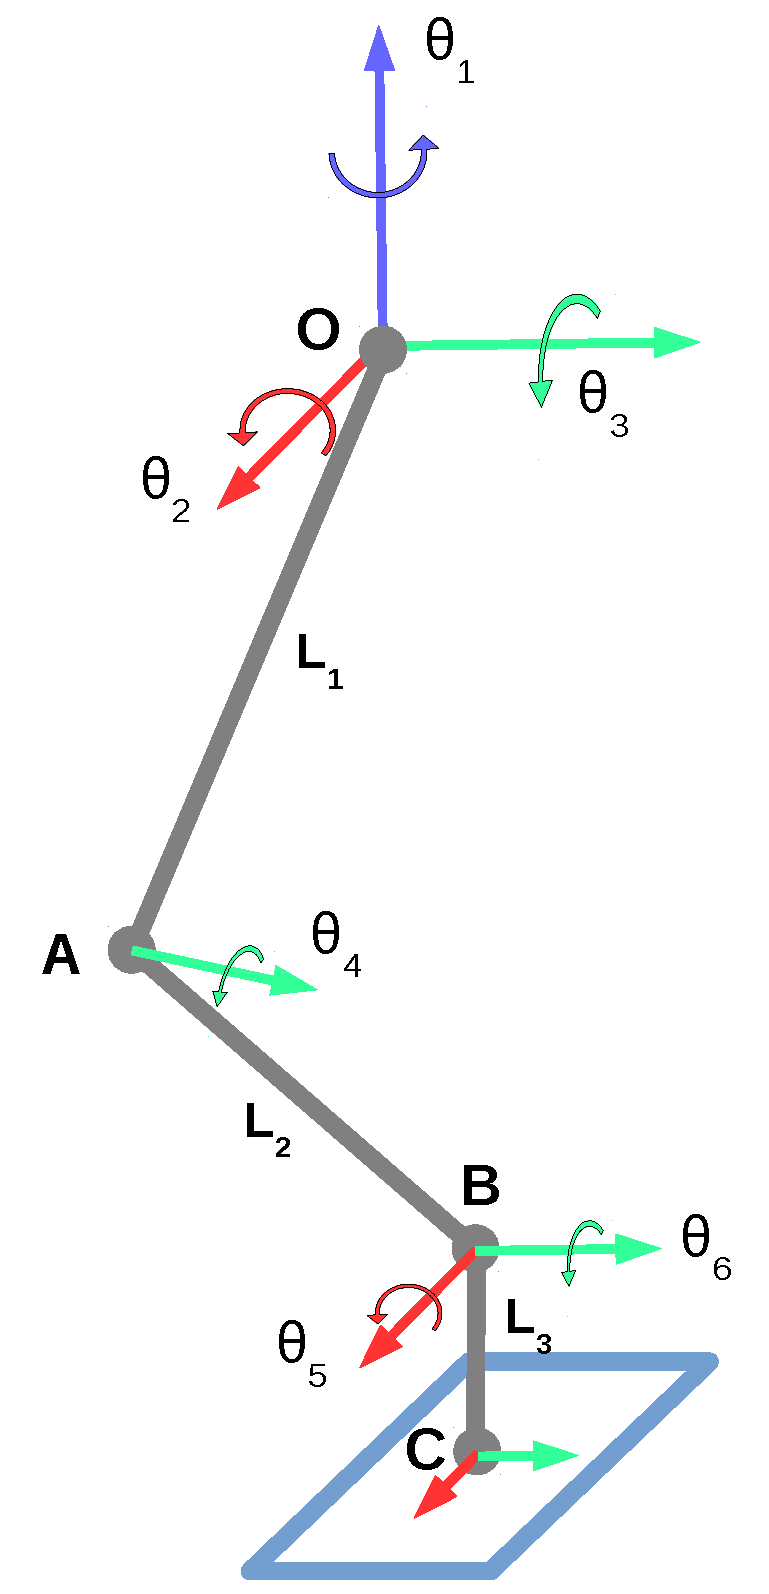
\includegraphics[type=pdf,ext=.pdf,read=.pdf,width=0.25\linewidth]{../schema/leg_ik}
        \caption{\label{fig:leg_ik}Notations pour le calcul du modèle géométrique inverse de la jambe.}
    \end{center}
\end{figure}

\begin{definition}
    Dans la suite, le terme \og \textit{espace cartésien} \fg désigne le monde 
    tridimensionnel dans lequel évolue le système mécanique du robot.
    Plus précisément, ce terme est selon les cas employé avec l'une 
    des deux significations suivante :
    Dans la première, il représente l'espace de dimension $3$ ($\mathbb{R}^3$)
    de l'ensemble des positions du monde. On considère alors
    un point dans l'espace tridimensionnel.
    Dans la seconde, il représente l'espace de dimension $6$ ($SO(3) \times \mathbb{R}^3$)
    des orientations et des positions. On considère dans ce cas un point associé à un
    repère orienté dans le monde tridimensionnel.
\end{definition}

Le modèle géométrique direct permet, à partir de l'état des degrés de liberté du
système dans l'espace articulaire, d'associer à tous les segments mécaniques
du robot\footnote{On considère plus précisément les repères liés à chaque segment}, 
une position et une orientation dans le monde tridimensionnel.
Le \textit{modèle géométrique inverse} réalise sur un robot polyarticulé 
\og partiellement \fg l'opération contraire :

\begin{definition}
    On considère un sous ensemble des segments mécaniques du robot, et on associe
    à chacun d'eux une contrainte soit de position, soit d'orientation, 
    soit des deux dans l'espace tridimensionnel.
    Par définition, le modèle géométrique inverse est la procédure calculant 
    l'ensemble des sous ensembles des degrés de liberté du système, tel que le
    système mécanique respecte toutes les contraintes cartésiennes définies,
    si cela est possible.
    L'ensemble des points (et des orientations) de l'espace cartésien
    pour lesquels il existe au moins une solution est appelé l'espace (ou zone) 
    d'accessibilité (ou atteignable) du robot (sachant les contraintes imposées).
\end{definition}

L'intérêt du modèle inverse est de pouvoir concevoir les mouvements du robot
directement dans l'espace cartésien plutôt que dans l'espace articulaire.
Le plus souvent, les objectifs et les contraintes d'un mouvement s'expriment 
en effet plus naturellement dans l'espace cartésien.
Par contre, il est alors nécessaire de prendre en compte une contrainte 
supplémentaire : les limites de la zone d'accessibilité.

Alors que le modèle géométrique direct admet toujours une et une seule
solution, le modèle inverse peut selon les cas n'en avoir aucune 
(configuration inatteignable), une seule, un nombre fini ou infini de solutions 
(topologie cinématique redondante).
Dans le cas général, le modèle géométrique inverse d'un robot polyarticulé 
ne possède pas de procédure de calcule sous forme analytique.
Dans ce cas, un calcul numérique et itératif peut être alors mené.
Grâce à la jacobienne du système mécanique au point considéré,
le problème est transformé en un problème d'optimisation (minimisation).
Par exemple, on peut mentionner l'utilisation de l'algorithme de minimisation
non linéaire aux moindres carrés de Levenberg-Marquardt (\cite{more_levenberg-marquardt_1978}), 
pour implémenter un modèle géométrique inverse itératif du centre de masse du robot.
Ceci a permis la génération et l'expérimentation d'une marche
purement statique\footnote{Centre de masse à tout moment dans l'enveloppe 
convexe du ou des pieds au sol.} sur le robot Sigmaban.

Dans le cas du modèle inverse de la jambe de Sigmaban, le problème est
bien posé : en fixant la position et l'orientation dans l'espace cartésien 
du centre du pied, $6$ contraintes sont imposées. Or, la jambe compte 
également $6$ degrés de liberté. 
Une solution analytique, bien plus performante en terme de temps de calcul est possible.
Le modèle géométrique inverse de la jambe admet donc : 
soit zéro solution si le point est en dehors de la zone d'accessibilité,
soit une seule solution au niveau de la singularité du robot jambe tendu, 
soit deux solutions dans le reste des cas.
Dans ces derniers cas, les deux solutions symétriques correspondent 
aux deux sens possibles de \og pliage \fg du genoux.
En imposant que le genoux ne se plie que de manière anthropomorphe, 
\og vers l'avant \fg, la solution du modèle géométrique inverse dans
sa zone d'accessibilité se réduit à une unique configuration des articulations.

L'implémentation du modèle géométrique inverse de la jambe de Sigmaban
(et de Grosban) sur laquelle nous nous sommes basés est disponible à l'adresse :\\
\url{https://github.com/RhobanProject/Model/tree/master/LegIK}\\
Les positions angulaires des $6$ degrés de liberté de la jambe 
sont calculées au travers d'une approche géométrique (voir la figure \ref{fig:leg_ik}).
Le code est écrit en C++ et une notice détaillant les étapes de résolution 
de la méthode est disponible.
À noter que dans ce code, le centre des axes de rotation de la hanche
est choisi comme repère de référence.
Cette implémentation est ensuite intégrée au reste de la gestion
des modèles géométriques pour en rendre son utilisation 
plus flexible dans n'importe quel repère.\\

Au code existant a été rajouté la fonctionnalité suivante :
Dans le cas général, il est difficile de calculer la distance la plus 
courte à l'enveloppe de la zone d'accessibilité (potentiellement non connexe).
Ici, une simple \og métrique \fg, sans unité, a été introduite.
Cette métrique estime un score d'autant plus grand que la configuration
cartésienne demandée n'est pas réalisable.
Plus précisément, le calcul du modèle géométrique inverse fait
intervenir de nombreuses conditions testant les cas limites.
Par exemple, certaines distances calculées doivent être non nulles, 
les valeurs aux entrées des fonctions trigonométriques inverses ($arccos$)
doivent être comprises entre $-1$ et $1$ pour qu'une solution existe.
Au moment de chacun de ces tests, au sein de l'implémentation, 
la distance à la contrainte numérique est calculée, 
sans aucun coefficient de normalisation.
La distance (signée) maximum est alors renvoyée par la procédure
de calcul du modèle inverse.
Ce critère simple n'a aucune signification physique, il n'est pas proportionnel 
à la distance à l'enveloppe d'accessibilité et il ne représente pas non plus
la distance la plus courte.
Néanmoins, il est d'une aide très importante pour la synthèse de mouvement
par optimisation. En donnant une direction au gradient, ce critère accélère
significativement la recherche d'un mouvement respectant les contraintes 
d'accessibilité imposées par le modèle géométrique inverse.\\

Pour résumer, le modèle géométrique inverse de la jambe se représente ainsi :
\begin{definition}
    Soit $\bm{p}_{\text{cible}} \in \mathbb{R}^3$ et
    $\bm{R}_{\text{cible}} \in SO(3)$ respectivement la position et l'orientation
    cartésienne cible du centre du pied.
    Le modèle géométrique inverse de la jambe est définie par 
    la procédure de calcul suivante :
    $$
    \mathsf{IK} :~ (\bm{p}_{\text{cible}}, \bm{R}_{\text{cible}}) 
    \longmapsto 
    (v, \bm{q}_{\text{jambe}}, d) 
    $$
    avec $v \in \{0,1\}$ une variable binaire indiquant si le modèle inverse
    admet ($1$) ou non ($0$) une solution.
    Si une solution existe, alors $\bm{q}_{\text{jambe}} \in \mathbb{R}^6$ 
    est le vecteur calculé des positions articulaires de la jambe.
    Enfin, $d \in \mathbb{R}$ est la métrique représentant la \og distance \fg
    à la zone d'accessibilité.
    Si $v = 0$, $d < 0$, sinon, $d \geqslant 0$.
\end{definition}

Bien qu'il ne soit pas détaillé ici, le modèle géométrique inverse 
de la tête du robot a également été implémenté.
Plus simple que pour les jambes, il s'agit de calculer les positions
angulaires du cou (deux degrés de liberté) pour que le centre optique 
de la caméra vise un point donné sur le sol.
Associé à l'odométrie, il est par exemple ainsi possible de suivre du regard 
un point fixe sur le sol tout en se déplaçant.

\subsection{Estimation de l'état géométrique du robot\label{sec:estimation_etat}}

À tout moment au cours de son fonctionnement, le robot enregistre 
et estime son état géométrique aux travers de ses différents capteurs.
La grande majorité des petits robots humanoïdes similaires à notre 
plateforme Sigmaban possèdent au moins les capteurs suivants :
\begin{itemize}
    \item Des encodeurs situés au niveau de chaque articulation
        mesurent la position angulaire absolue des articulations.
    \item Une centrale inertielle habituellement placée dans le buste
        du robot fournit à l'aide d'accéléromètres une orientation
        absolue par rapport au vecteur vertical de gravité.
        Des gyromètres mesurent également les vitesses de rotation
        instantanées autour des axes locaux du robot.
\end{itemize}

Les centrales inertielles peuvent également être équipées de 
magnétomètres estimant la direction du champ magnétique local. 
Dans de bonnes conditions, le magnétomètre permet de connaitre 
le sens du champ magnétique terrestre et ainsi d'accéder à un
azimut absolu dans le monde.

Malheureusement en pratique, le champ magnétique est fortement 
perturbé par les masses métalliques du robot, par les variations 
de courant au sein des bobines des moteurs à courant
continu ainsi que par l'environnent magnétique du terrain lui même. 
La direction du Nord magnétique mesurée est alors très bruitée.
Selon les cas, l'erreur d'orientation peut varier entre $10$ et $50$ degrés.
Néanmoins, certaines équipes de la RoboCup humanoïde ont parfois 
mis en oeuvre des procédures de calibration du magnétomètre
voire même de cartographie du champs magnétique du terrain.

A partir de l'édition 2017, l'évolution du règlement de la ligue 
humanoïde\footnote{Le règlement de la ligue humanoïde 
RoboCup est disponible ici : \url{https://www.robocuphumanoid.org/materials/rules/}}
rend l'utilisation du magnétomètre illégale dans l'objectif de ne strictement 
autoriser que les capteurs ayant un équivalent chez l'humain.

À noter que ces robots \og type RoboCup \fg possèdent aussi
une caméra au niveau de la tête. 
Potentiellement, l'analyse visuelle peut également fournir une donnée
d'orientation absolue (azimut et assiette par rapport à l'horizon)
(voir la bibliographie de l'odométrie visuelle à la section \ref{sec:biblio_odometry}).
La caméra est le capteur fournissant le plus d'informations mais également
le plus difficile à analyser rapidement et de manière robuste.
Dans la suite, la caméra n'est utilisée que pour la reconnaissance 
d'éléments extérieurs et non pour l'estimation de l'état du 
robot (hors localisation absolue).\\

La centrale inertielle située à la base du buste du robot
fournit au travers du bus de communication les valeurs brutes
des accéléromètres et des gyromètres.
Très souvent, on leur préfère une estimation filtrée en unités SI.

Les accéléromètres et les gyromètres utilisés sont des
micro-systèmes électromécaniques (\textit{Microelectromechanical Systems} ou MEMS)
mesurant tous deux des micros déplacements de masses tests sous l'effet de forces.

Les accéléromètres évaluent les forces linéaires appliquées 
au capteur selon les trois axes de l'espace.
Le but étant de mesurer la direction du vecteur de gravité et d'en
déduire l'orientation absolue du robot par rapport à la verticale.
Malheureusement, les accélérations ou les vibrations latérales
du robot sont également enregistrées et ne peuvent
être distinguées de la mesures du champ de gravité.
Ainsi, on considère que les accéléromètres sont soumis
à un bruit haute fréquence mais converge au repos vers 
une valeur de précision acceptable du vecteur de gravité.

D'un autre coté, les gyromètres à l'aide de mesures différentielles 
des forces de Coriolis estiment les vitesses de rotation
instantanées autour des axes de l'espace. 
Leurs mesures différentielles ne sont que peu affectées par 
les accélérations de translations mais elle souffrent d'un défaut 
de résilience. La référence \textit{zéro} de ces MEMS tend à dériver
lentement de sorte que même au repos, un gyromètre mesure souvent une
faible vitesse de rotation mais non nulle. Ils sont considérés comme
soumis à une erreur basse fréquence mais relativement juste 
à haute fréquence.

Il est ainsi très courant de filtrer et de mélanger les mesures
de ces deux capteurs afin d'obtenir une estimation corrigée de
l'orientation en unités SI.
Ce système est appelé \og centrale de cap et d'attitude \fg 
AHRS (\textit{Attitude and Heading Reference System}).

Trois grandes familles de filtres sont couramment mises en 
oeuvre\footnote{Une introduction à ces différents filtres
est disponible en ligne par OlliW Bastelseiten : \url{http://www.olliw.eu/2013/imu-data-fusing/}} :
\begin{itemize}
    \item Le filtre de Kalman : il s'agit du filtre générique classique optimal
        dans le cas linéaire avec des bruits gaussiens (\cite{grewal2011kalman}). 
        Le modèle de transition prédit l'orientation courante à partir de 
        l'ancienne orientation et de l'intégration des vitesses de rotation
        mesurées par les gyromètres. 
        L'incertitude sur l'état est mise à jour et représentée sous forme 
        d'une distribution gaussienne multivariée.
        Ensuite, la prédiction est mélangée à la mesure de l'orientation
        donnée par les accéléromètres afin de corriger sa dérive.
        La matrice des gains optimale effectuant la pondération est recalculée
        en permanence en prenant en compte les incertitudes sur l'état courant.
        À noter que l'intégration des rotations de l'espace est 
        un calcul non linéaire. 
        La version étendue (\textit{Extended Kalman Filter}) 
        de la théorie de Kalman par linéarisation successive 
        doit alors être utilisée.
    \item Le filtre complémentaire : il s'agit en réalité d'une simplification
        du filtre de Kalman (\cite{higgins1975comparison}) 
        très utilisé par la communauté des \og hobbyistes \fg.
        En effet, le filtre de Kalman étendu est délicat à implémenter
        sur des petits micro contrôleurs 8 bits.
        Le gain de pondération de la phase d'observation du filtre de Kalman
        est supposé constant et l'incertitude sur l'état n'est pas considérée.
        Le filtre se réduit alors à un filtre passe haut intégrant rapidement 
        les vitesses de rotation du gyromètre et à un filtre passe bas convergeant 
        lentement vers l'orientation estimée par les accéléromètres.
    \item Le filtre de Mahony : contrairement aux précédents, le filtre de Mahony
        (\cite{mahony_nonlinear_2008}, \cite{euston_complementary_2008}) cible
        spécifiquement le problème du filtrage de l'orientation à partir d'IMU MEMS.
        Les rotations de l'espace sont soit représentées par des matrices de rotation
        (ou matrice de cosinus directeur, DCM), soit par des quaternions.
        Ce filtre se base sur les même principes que le filtre complémentaire mais
        ajoute une correction explicite de la dérive du gyromètre.
        Son implémentation sur de petits micro contrôleurs est 
        également abordée.
\end{itemize}

À noter que le filtre de 
Madwick\footnote{L'implémentation du filtre de Mahony ainsi que du filtre 
de Madwick par est maintenue ici par Sebastian Madgwick : \url{http://x-io.co.uk/open-source-imu-and-ahrs-algorithms/}}
(\cite{madgwick_efficient_2010}, \cite{madgwick_estimation_2011})
est également très utilisé dans le filtrage des centrales inertielles MEMS.
Mais à la différence des méthodes détaillées ci-dessus, le filtre de Madwick s'intéresse
aux IMU à 9 degrés de liberté utilisant le magnétomètre pour estimer également un azimut absolu.\\

À bord du robot Sigmaban, la centrale inertielle est filtrée au niveau de son
ordinateur embarqué par une implémentation dérivée du filtre 
de Mahony\footnote{Autre implémentation du filtrage se basant sur les travaux de Mahony par Peter Bartz 
ciblant originellement les IMU \textit{Razor AHRS}  : \url{https://github.com/Razor-AHRS/razor-9dof-ahrs}.
La version utilisée à bord de Sigmaban a été modifiée afin d'être intégrée 
à la bibliothèque bas niveau de Rhoban et s'exécuter sur le calculateur principal du robot.}.
Ce filtre permet de déterminer le roulis et le tangage du robot par rapport à la verticale.

Sans l'utilisation de magnétomètres et malgré la dérive inévitable, l'intégration
pure des gyromètres autour de l'axe vertical permet néanmoins d'obtenir une
estimation relative du lacet (ou azimut) du robot dans le monde. 
Sans référence absolue, l'azimut est alors donné par 
rapport à l'orientation initiale.
À noter que le moyennage au repos des mesures des gyromètres permet
une calibration rapide compensant temporairement la non résilience des MEMS.
Ainsi, l'estimation absolue de l'azimut du robot dans le monde par pure
intégration reste acceptable pour nos besoins sur une durée de l'ordre
de quelques minutes\footnote{Il est donc recommandé d'effectuer la calibration 
des gyromètres à chaque démarrage du robot.}.

Le filtre de l'IMU renvoie ainsi l'orientation
absolue du buste du robot $\bm{R}_{\text{IMU}} \in SO(3)$ dans le monde 
par rapport à la verticale et par rapport à l'azimut initial.\\

En supposant le pied de support à plat sur le sol, 
la cinématique directe de la jambe détermine l'orientation 
du buste du robot.
Mais en pratique, on constate souvent un écart de quelques
degrés entre l'orientation fournie par la cinématique et 
la mesure d'orientation de l'IMU.
Ceci est dû d'une part au jeu mécanique des articulations 
non mesuré par les encodeurs des moteurs ainsi qu'au
montage de l'IMU qui n'est pas parfaitement alignée avec les 
axes du robot.
Malheureusement, il n'est pas possible de mélanger ces deux mesures
pour améliorer la précision puisque sur l'herbe artificielle ou lors
d'une chute, le pied de support du robot n'est pas plat par rapport au sol.
Il pourrait d'ailleurs être intéressant d'installer des centrales inertielles
au niveau des pieds du robot pour acquérir cette information.

En conséquence, l'orientation donnée par la cinématique et par l'IMU sont toutes
deux considérées correctes. 
L'écart observé entre ces deux mesures est alors expliqué par l'inclinaison
du pied sur le sol.
Plus précisément, l'idée est alors d'utiliser les deux degrés de liberté 
de la base flottante \textit{base\_roll} et \textit{base\_pitch}
afin d'incliner le pied par rapport au plan du sol de sorte que l'orientation
du buste du robot coïncide avec la mesure de l'IMU.\\

La fréquence de la boucle bas niveau de lecture écriture 
est variable et tourne au alentour de $100$~Hz.
À chaque cycle, la position courante de tous les moteurs ainsi
que les valeurs brutes des accéléromètres et gyromètres sont
lus et le filtrage appliqué. 
Le modèle est alors mis à jour comme suit :
\begin{itemize}
    \item La position angulaire $q_i$ de toutes les articulations
        est donnée par la position lue par les encodeurs absolus des moteurs.
    \item Le centre du pied le plus bas dans le repère du monde 
        est supposé en contact avec le sol et détermine le pied de support.
        $$
        h_{\text{left\_foot}} = 
        \mathsf{FK}_{\text{position}}(\bm{q}, \bm{0}, \mathfrak{R}_{\text{left\_foot\_tip}}, \mathfrak{R}_{o}).\vec{\bm{z}}
        $$
        $$
        h_{\text{right\_foot}} = 
        \mathsf{FK}_{\text{position}}(\bm{q}, \bm{0}, \mathfrak{R}_{\text{right\_foot\_tip}}, \mathfrak{R}_{o}).\vec{\bm{z}}
        $$
        Si $h_{\text{left\_foot}} \leqslant h_{\text{right\_foot}}$ alors 
        le pied gauche ($LSS$) est le pied de support, sinon il s'agit du pied droit ($RSS$). 
    \item L'orientation en roulis et tangage du pied par rapport au sol
        est choisie telle que l'orientation du buste du robot soit en accord avec celle fournie
        par la centrale inertielle. 
        L'orientation en lacet est calculée par pure intégration
        des gyromètres autour de la verticale.
        $$
        \bm{R}_{\text{origin}}^{\text{trunk}} = \bm{R}_{\text{IMU}} \in SO(3)
        $$
        $$
        \bm{R}_{\text{trunk}}^{\text{foot}} = 
        \mathsf{FK}_{\text{orientation}}(\bm{q}, \mathfrak{R}_{\text{trunk}}, \mathfrak{R}_{\text{foot}})
        \in SO(3)
        $$
        $$
        \bm{R}_{\text{origin}}^{\text{foot}} = 
        \bm{R}_{\text{trunk}}^{\text{foot}}~.~
        \bm{R}_{\text{origin}}^{\text{trunk}}
        $$
        L'orientation du pied de support par rapport au monde est ensuite décomposé 
        en angles de Cardan (voir annexe \ref{sec:angles_euler}) et
        assignés aux degrés de liberté de la base flottante.
        $$
        \begin{bmatrix}
        \theta_{\text{roll}} \\
        \theta_{\text{pitch}} \\
        \theta_{\text{yaw}} \\
        \end{bmatrix}
        =
        \mathsf{MatrixToCardan}(\bm{R}_{\text{origin}}^{\text{foot}})
        \in \mathbb{R}^3
        $$
        $$
        q_{\text{base\_roll}} = \theta_{\text{roll}},~~
        q_{\text{base\_pitch}} = \theta_{\text{pitch}},~~ 
        q_{\text{base\_yaw}} = \theta_{\text{yaw}}
        $$
\end{itemize}

\subsection{Calculs et conventions odométriques\label{sec:def_odometry}}

L'odométrie a pour objet l'estimation 
des déplacements du robot dans le monde relativement 
à un point de départ, au travers des mesures des capteurs
et des ordres donnés au mouvement de marche.
Ce paragraphe présente le calcul classique des déplacements
relatifs à partir de l'intégration de la cinématique des jambes.
Cette estimation est développée et étendue dans la section \ref{sec:odometry_intro}.

Pour parler de la position et de l'azimut du robot sur le plan du sol,
on défini le repère égocentrique $\mathfrak{R}_{\text{self}}$ lié au robot.

\begin{definition}
Le repère égocentrique du robot $\mathfrak{R}_{\text{self}}$
n'est pas lié à un solide mais se construit à partir du repère
\textit{trunk} situé à la base du buste.
Le centre $O_{\text{self}}$ du repère égocentrique est la projection
sur le sol (plan $(O,\bm{\vec{x}},\bm{\vec{y}})$)) 
de l'origine du repère \textit{trunk}.
L'orientation du repère égocentrique se construit en appliquant
une rotation d'axe $\bm{\vec{z}}$ au repère de référence 
à l'origine du monde.
L'angle de cette rotation est tel que l'axe $\bm{\vec{x}}_{\text{trunk}}$ du repère lié au buste du robot
soit dans le plan $(O_{\text{self}}, \bm{\vec{x}}_{\text{self}}, \bm{\vec{z}}_{\text{self}})$ 
et que $\bm{\vec{x}}_{\text{trunk}}.\bm{\vec{x}}_{\text{self}} > 0$.
\end{definition}
Le repère égocentrique est \og plat \fg par rapport au sol, situé sur le plan du sol 
et pointe vers l'avant du robot. L'azimut se calcule par la décomposition en angle
de Cardan de l'orientation du buste exprimée dans le repère du monde.\\

L'attitude ou pose du robot dans le monde est par définition 
représentée par le vecteur : 
$$
\bm{p} = \begin{bmatrix}x \\ y \\ \theta \end{bmatrix} =
\begin{bmatrix}
\mathsf{FK}_{\text{position}}(\bm{q}, \bm{0}, \mathfrak{R}_{\text{self}}, \mathfrak{R}_{o}).\vec{\bm{x}} \\
\mathsf{FK}_{\text{position}}(\bm{q}, \bm{0}, \mathfrak{R}_{\text{self}}, \mathfrak{R}_{o}).\vec{\bm{y}} \\
\mathsf{MatrixToCardan}(\mathsf{FK}_{\text{orientation}}(\bm{q}, \mathfrak{R}_{\text{self}}, \mathfrak{R}_{o})).\vec{\bm{z}}
\end{bmatrix}
\in \mathbb{R} \times \mathbb{R} \times ]-\pi,\pi]
$$\\

La mise à jour du modèle à partir des mesures des capteurs,
présentée dans la section précédente, permet d'intégrer au cours
du temps l'état du robot dans le monde.

Comme indiqué à la section \ref{sec:support_foot}, le robot 
est en réalité modélisé à l'aide de deux arbres géométriques.
Durant les phases de support gauche (respectivement droit), 
l'arbre utilisé est celui dont la racine (virtuelle) est 
attachée au centre du pied gauche (respectivement droit).

Au moment de la transition du pied de support, l'arbre courant 
est échangé et le nouveau modèle est mis à jour. 
Ici, \textit{flying foot} fait référence au centre de l'autre pied 
sur le point de devenir le nouveau pied de support :
\begin{itemize}
    \item Les positions de toutes les articulations sont copiées 
        de l'arbre de l'ancien support vers l'arbre du nouveau support.
    \item Afin d'assurer la continuité des positions des solides du robot dans 
        le repère du monde, la nouvelle base flottante est mise à jour comme suit :
        $$
        \mathfrak{R}_{\text{flying foot}} \in \{\mathfrak{R}_{\text{left\_foot\_tip}}, \mathfrak{R}_{\text{left\_foot\_tip}}\}
        $$
        $$
        \bm{p}_{\text{flying foot}} = 
        \mathsf{FK}_{\text{position}}(\bm{q}, \bm{0}, \mathfrak{R}_{\text{flying foot}}, \mathfrak{R}_{o})
        $$
        $$
        q_{\text{base\_x}} = \bm{p}_{\text{flying foot}}.\vec{\bm{x}},~~
        q_{\text{base\_y}} = \bm{p}_{\text{flying foot}}.\vec{\bm{y}}
        $$
        $$
        q_{\text{base\_yaw}} = 
        \mathsf{MatrixToCardan}(
        \mathsf{FK}_{\text{orientation}}(\bm{q}, \mathfrak{R}_{\text{flying foot}}, \mathfrak{R}_{o})
        ).\vec{\bm{z}}
        $$
    \item Enfin, l'inclinaison du nouveau pied de support par rapport au sol 
        est mise à jour à partir de l'IMU comme précisé dans la section précédente.
\end{itemize}

À chaque changement de pied de support, les degrés de liberté de la base 
flottante attachée au pied du robot sont ainsi discontinus.
Grâce à cette intégration de la position du pied de support au cours du temps, 
la pose du robot dans le monde est continue et calculable à chaque 
instant au travers du repère égocentrique.\\

\begin{figure}[htb]
    \begin{center}
        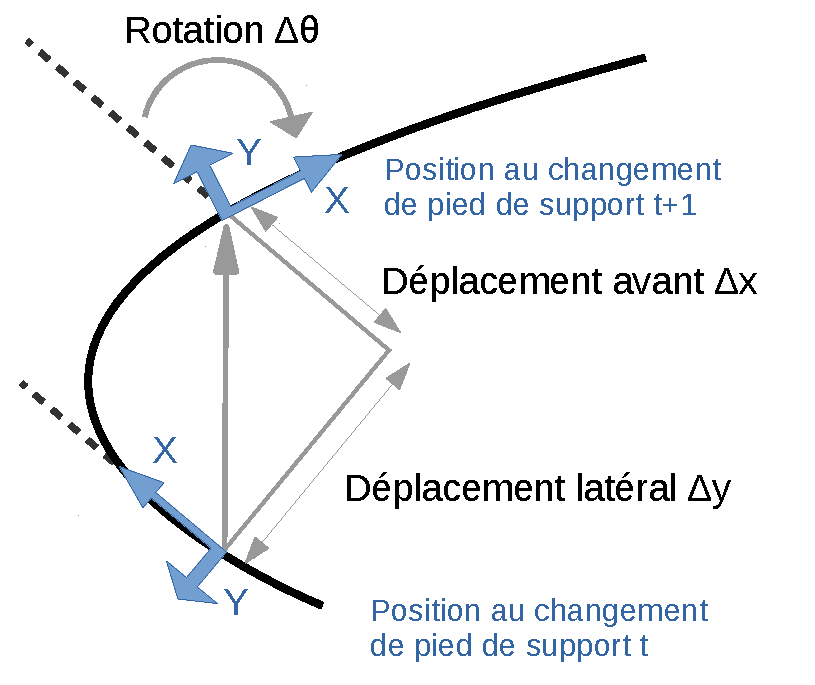
\includegraphics[type=pdf,ext=.pdf,read=.pdf,width=0.6\linewidth]{../schema/footstep}
        \caption{\label{fig:footstep}
            Modèle de déplacement en translation et en rotation du robot 
            entre deux transitions de pied de support.}
    \end{center}
\end{figure}

Le déplacement du robot entre deux changements de pied 
de support correspond à un pas (un demi cycle de marche) 
et se note 
$\Delta \bm{p} = \begin{bmatrix}\Delta x \\ \Delta y \\ \Delta \theta\end{bmatrix} \in \mathbb{R}^3$.
Par convention, ce déplacement est exprimé dans le repère
égocentrique du robot.
Plus précisément, la figure~\ref{fig:footstep} dépeint la transformation géométrique planaire.
La translation de vecteur $\begin{bmatrix}\Delta x \\ \Delta y\end{bmatrix}$ exprimée dans le
repère égocentrique de départ est appliquée en premier. 
La rotation d'angle $\Delta \theta$ est appliquée en second.\\

La pose du robot (exprimé dans le repère du monde) à deux changements de pied 
support successifs est notée $\bm{p}_{t}$ et $\bm{p}_{t+1}$.
On définie alors les deux fonctions $\mathsf{displacementInt}$ et $\mathsf{displacementDiff}$
utilisées dans la suite par les relations suivantes :
$$
\bm{p}_{t+1} = \mathsf{displacementInt}\big(\bm{p}_{t}, \Delta \bm{p}_{t}\big)
$$
et inversement :
$$
\Delta \bm{p}_{t} = \mathsf{displacementDiff}\big(\bm{p}_{t}, \bm{p}_{t+1}\big)
$$

La première intègre la pose du robot à partir du vecteur du déplacement relatif.
La seconde calcule le déplacement relatif sachant deux poses successives.
Enfin, ces deux fonctions se construisent de la manière suivante :

\begin{gather*}
\mathsf{displacementDiff} : 
\big(\begin{bmatrix}x_{t} \\ y_{t} \\ \theta_{t}\end{bmatrix},
\begin{bmatrix}x_{t+1} \\ y_{t+1} \\ \theta_{t+1}\end{bmatrix}\big)
\longmapsto \\
\Delta \bm{p}_{t} = \begin{bmatrix}\Delta x \\ \Delta y \\ \Delta \theta \end{bmatrix}
= 
\begin{bmatrix} 
\bm{R}_{\text{2d}}(-\theta_{t})\begin{bmatrix}x_{t+1}-x_{t} \\ y_{t+1}-y_{t}\end{bmatrix} \\ 
\mathsf{angleDistance}(\theta_{t}, \theta_{t+1}) 
\end{bmatrix}
\end{gather*}

\begin{gather*}
\mathsf{displacementInt} : 
\big(\begin{bmatrix}x_{t} \\ y_{t} \\ \theta_{t}\end{bmatrix},
\begin{bmatrix}\Delta x \\ \Delta y \\ \Delta \theta\end{bmatrix}\big)
\longmapsto \\
\bm{p}_{t+1} = \begin{bmatrix}x_{t+1} \\ y_{t+1} \\ \theta_{t+1}\end{bmatrix}
= 
\begin{bmatrix}
\begin{bmatrix}x_{t} \\ y_{t}\end{bmatrix} + \bm{R}_{\text{2d}}(\theta_{t})\begin{bmatrix}\Delta x \\ \Delta y\end{bmatrix}\\
\mathsf{angleBound}(\theta_{t} + \Delta \theta) 
\end{bmatrix}
\end{gather*}

\subsection{Implémentation\label{sec:model_geometric_rbdl}}

La figure \ref{fig:model_gui} montre notre outil de représentation 
graphique du modèle.
La modélisation géométrique (et dynamique) de nos robots 
humanoïdes est réalisée en C++ et peut être consultée à l'adresse :\\
\url{https://github.com/RhobanProject/Model}.\\

Cette implémentation est construite à l'aide de la bibliothèque 
\textit{RBDL} (\textit{Rigid Body Dynamics Library}) écrite par Martin Felis.
Son code source est librement disponible à l'adresse :\\
\url{https://bitbucket.org/rbdl/rbdl/}.\\

Les algorithmes mis en oeuvre, les notations et la représentation interne des données de RBDL 
suivent fidèlement le livre de référence \og \textit{Rigid Body Dynamics Algorithm} \fg
de Roy Featherstone, \cite{featherstone_rigid_2008}.

\begin{figure}[htb]
    \centerfloat
    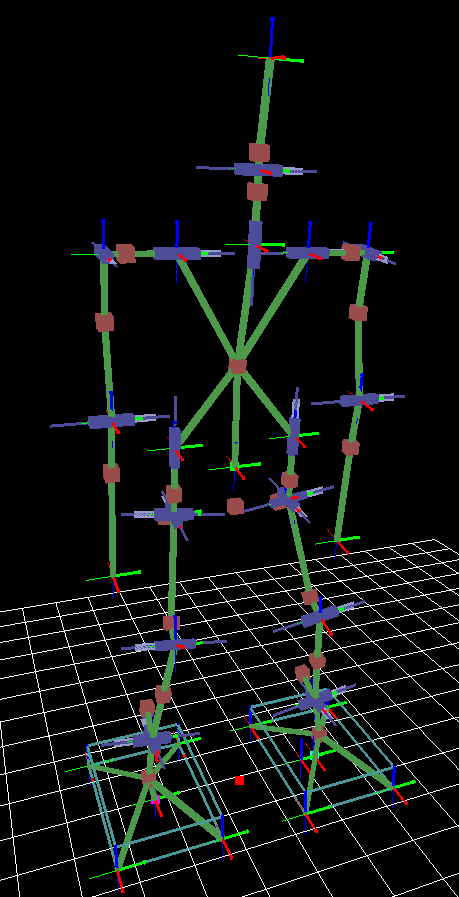
\includegraphics[height=9cm]{../media/model_gui1.png}
    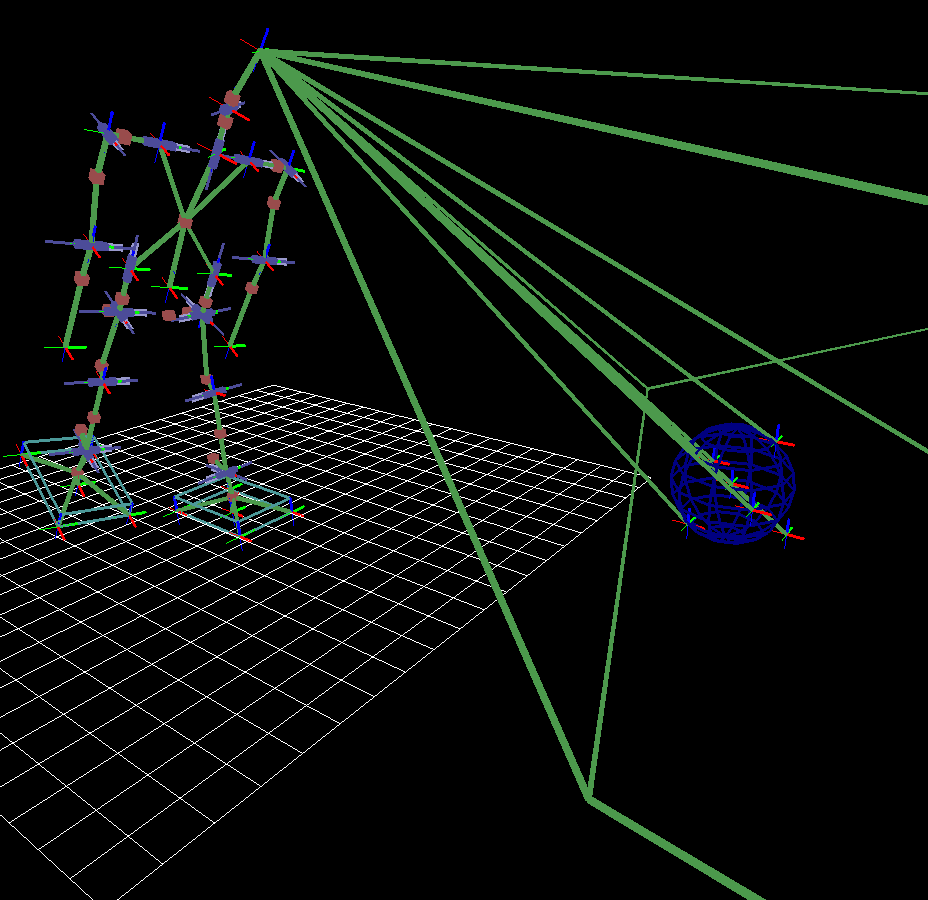
\includegraphics[height=9cm]{../media/model_gui2.png}
    \caption{\label{fig:model_gui} 
        Visualisation graphique (OpenGL)
        de l'implémentation du modèle géométrique de Sigmaban.
        Les articulations sont représentées par un cylindre bleu
        et les centres de masse de chaque segments mécaniques
        par un cube rouge.
        Sur chaque pièce mécanique est également affiché le repère local associé.
        À droite, le trapézoïde du modèle de caméra du robot visant une balle 
        sur le sol est représenté.
    }
\end{figure}

